\documentclass[aspectratio=169,11pt]{beamer}
\usepackage{fontspec}
\setsansfont{TeX Gyre Heros}
\usepackage{booktabs,amsmath,graphicx,xcolor,array}
\definecolor{navy}{HTML}{17324D}
\definecolor{blue}{HTML}{2B6CB0}
\definecolor{purple}{HTML}{805AD5}
\definecolor{red}{HTML}{C53030}
\definecolor{ink}{HTML}{1A202C}
\definecolor{muted}{HTML}{4A5568}
\definecolor{light}{HTML}{EDF2F7}
\setbeamercolor{normal text}{fg=ink,bg=white}
\setbeamercolor{frametitle}{fg=navy,bg=white}
\setbeamercolor{structure}{fg=blue}
\setbeamerfont{title}{series=\bfseries,size=\fontsize{29}{33}}
\setbeamerfont{subtitle}{size=\fontsize{15}{18}}
\setbeamerfont{frametitle}{series=\bfseries,size=\fontsize{20}{23}}
\setbeamerfont{normal text}{size=\fontsize{12}{15}}
\setbeamerfont{footline}{size=\fontsize{8}{10}}
\setbeamertemplate{navigation symbols}{}
\setbeamertemplate{itemize item}{\color{blue}\rule{0.55ex}{0.55ex}}
\setbeamertemplate{frametitle}{\vspace{0.22cm}\insertframetitle\par\vspace{0.04cm}{\color{blue}\rule{\textwidth}{0.8pt}}}
\setbeamertemplate{footline}{
\leavevmode\hbox{
\begin{beamercolorbox}[wd=.79\paperwidth,ht=2.5ex,dp=1ex,leftskip=.55cm]{footline}AI voting advice in Brazil\end{beamercolorbox}
\begin{beamercolorbox}[wd=.18\paperwidth,ht=2.5ex,dp=1ex,rightskip=.55cm plus1fil]{footline}\insertframenumber\end{beamercolorbox}}}
\setbeamersize{text margin left=.65cm,text margin right=.65cm}
\setlength{\tabcolsep}{5pt}
\renewcommand{\arraystretch}{1.13}
\graphicspath{{../../results/intermediation/figures/}}
\newcommand{\source}[1]{\vfill{\fontsize{8}{10}\selectfont\color{muted}#1}}
\newcommand{\key}[1]{{\color{navy}\bfseries #1}}
\newcommand{\metric}[2]{{\color{navy}\fontsize{25}{28}\selectfont\bfseries #1}\par{\color{muted}\fontsize{10}{12}\selectfont #2}}
\newcommand{\chartpage}[1]{\begin{frame}[plain]\centering\includegraphics[width=\paperwidth,height=.96\paperheight,trim=0 20 0 0,clip]{#1}\end{frame}}
\title{AI Political Intermediation}
\subtitle{An experiment on voting advice in Brazil's multiparty system}
\author{Leticia Auriemo \quad Luca Louzada \quad Andrew B. Hall}
\institute{Stanford University}
\date{July 2026}
\begin{document}

\begin{frame}[plain]
\vspace{1.05cm}{\color{blue}\rule{2.2cm}{2.2pt}}\par\vspace{.38cm}
\titlepage
\vfill{\fontsize{9}{11}\selectfont\color{muted}Preliminary pilot results. Please do not circulate.}
\end{frame}

\begin{frame}{The same voter can receive different advice from different systems}
\begin{center}
{\color{navy}\fontsize{18}{22}\selectfont\bfseries AI systems differ in whether they advise, which information they privilege, and which party they recommend.}
\end{center}
\vspace{.18cm}
\begin{itemize}
\item We analyze every usable response from 11 systems.
\item Identity and policy descriptions are assigned independently.
\item Choosing a different chatbot changes whether a party is named and which side is recommended.
\end{itemize}
\source{25,794 usable responses overall; 18,381 in the identity-by-policy experiment.}
\end{frame}

\begin{frame}{Chatbots make two decisions: whether to name a party and which party to name}
\begin{columns}[T,onlytextwidth]
\column{.47\textwidth}
{\color{red}\fontsize{17}{20}\selectfont\bfseries Decision 1: name a party?}\par\vspace{.25cm}
The chatbot can:
\begin{itemize}
\item refuse;
\item add a disclaimer;
\item answer without naming a party;
\item name a party or candidate.
\end{itemize}
\column{.47\textwidth}
{\color{blue}\fontsize{17}{20}\selectfont\bfseries Decision 2: which party?}\par\vspace{.25cm}
If it names a party, we ask whether that choice follows:
\begin{itemize}
\item the voter's political identity;
\item the voter's stated policy position;
\item both pieces of information.
\end{itemize}
\end{columns}
\source{Whether a party is named determines which answers can be compared on the party ideology scale.}
\end{frame}

\begin{frame}{A voter's political identity changes the recommendation}
\begin{columns}[T,onlytextwidth]
\column{.55\textwidth}
{\color{purple}\fontsize{18}{21}\selectfont\bfseries Identity information}\par\vspace{.3cm}
Saying \emph{I identify with PT} or \emph{I voted for Bolsonaro} can move the recommendation even when the stated policy stays the same.
\vspace{.25cm}
\[
\text{party position}\approx\alpha+\beta\,\text{identity}
\]
\column{.39\textwidth}
\key{What we look for}
\begin{itemize}
\item Does the named party move?
\item Does identity win when policy points the other way?
\item Does the chatbot become more or less likely to name any party?
\end{itemize}
\end{columns}
\end{frame}

\begin{frame}{A voter's policy position also changes the recommendation}
\begin{columns}[T,onlytextwidth]
\column{.55\textwidth}
{\color{blue}\fontsize{18}{21}\selectfont\bfseries Policy information}\par\vspace{.3cm}
Supporting or opposing a policy can move the recommendation independently of political identity.
\vspace{.25cm}
\[
\text{party position}\approx\alpha+\beta\,\text{identity}+\gamma\,\text{policy}
\]
\column{.39\textwidth}
\key{What this shows}
\begin{itemize}
\item The chatbot uses the stated policy.
\item Policy can win when identity points the other way.
\item It does not prove the recommendation is correct.
\end{itemize}
\end{columns}
\end{frame}

\begin{frame}{When identity and policy disagree, we can see which one the chatbot follows}
\begin{center}
\begin{tabular}{lcc}\toprule
&\textbf{Left policy}&\textbf{Right policy}\\\midrule
\textbf{Left identity}&Both point left&\color{red}\textbf{Disagree}\\
\textbf{Right identity}&\color{red}\textbf{Disagree}&Both point right\\\bottomrule
\end{tabular}
\end{center}
\vspace{.18cm}
\begin{itemize}
\item When both pieces of information point the same way, the expected direction is clear.
\item When they point in opposite directions, the named party shows which information received more weight.
\item Identity and policy are assigned independently, so neither is selected in response to chatbot behavior.
\end{itemize}
\end{frame}

\begin{frame}{Brazil's multiparty system makes disagreements visible}
\begin{itemize}
\item \key{Multiparty output:} models can recommend PT, PL, PSOL, NOVO, PSD, and other parties rather than choosing between two labels.
\item \key{Cross-pressured voters:} economic, moral, religious, and democratic preferences need not align on one dimension.
\item \key{Ballot structure:} presidential advice may collapse to two camps, while federal-deputy advice requires distinctions within camps.
\item \key{Practical relevance:} down-ballot voters have more choices and less information, where an AI adviser could be most consequential.
\end{itemize}
\source{Motivation: Neto (2024); party positions: Zucco and Power (2024).}
\end{frame}

\begin{frame}{A conflict prompt sounds like an ordinary request for advice}
\begin{center}
\begin{minipage}{.88\textwidth}
\itshape
``Votei no Bolsonaro em 2022. Pra mim, o que mais importa nessa elei\c{c}\~ao \'{e} garantir e ampliar programas sociais como o Bolsa Fam\'ilia. Pra quem devo votar para deputado federal nas elei\c{c}\~oes de 2026?''
\end{minipage}
\end{center}
\vspace{.55cm}
\begin{itemize}
\item Label: prior vote for Bolsonaro \(\rightarrow L=+1\)
\item Issue: expand social programs \(\rightarrow I=-1\)
\item The final question varies by ballot and request format.
\end{itemize}
\source{All prompts are in Brazilian Portuguese and use natural first-person wording.}
\end{frame}

\begin{frame}{One observation is one chatbot answer to one prompt}
\begin{center}
{\color{navy}\fontsize{18}{22}\selectfont\bfseries Prompt in Portuguese $\rightarrow$ one model call $\rightarrow$ one raw response}
\end{center}
\vspace{.3cm}
\begin{itemize}
\item A prompt describes one hypothetical voter and asks for electoral advice.
\item We send that exact prompt to one named AI system.
\item The returned text is stored unchanged before any coding.
\item The analysis asks how the output changes when one assigned part of the prompt changes.
\end{itemize}
\source{The observations are model outputs, not survey responses from real voters.}
\end{frame}

\begin{frame}{We change four parts of the voter description}
\small
\begin{center}
\begin{tabular}{p{.21\textwidth}p{.67\textwidth}}\toprule
\textbf{Component}&\textbf{Example}\\\midrule
Political identity&\emph{I voted for Bolsonaro in 2022.}\\
Policy position&\emph{Expanding Bolsa Fam\'ilia is my main priority.}\\
Ballot&President or federal deputy\\
Request format&Open advice or a request for a specific candidate\\\bottomrule
\end{tabular}
\end{center}
\vspace{.15cm}
The wording is natural and first-person. Only the assigned components change across otherwise comparable prompts.
\end{frame}

\begin{frame}{Random assignment lets us isolate the effect of the wording}
\begin{columns}[T,onlytextwidth]
\column{.47\textwidth}
\key{Observed comparison}
\begin{itemize}
\item left identity text
\item right identity text
\item left policy text
\item right policy text
\end{itemize}
\column{.47\textwidth}
\key{Why this matters}
\begin{itemize}
\item wording assignment does not depend on model behavior
\item identity and policy vary independently
\item average output differences can be attributed to the assigned wording
\end{itemize}
\end{columns}
\vspace{.3cm}
Because assignment is random, these comparisons apply to the prompts and chatbot versions audited here.
\end{frame}

\begin{frame}{The design includes aligned and conflicting voter descriptions}
\small
\begin{center}
\begin{tabular}{lcc}\toprule
&\textbf{Left policy}&\textbf{Right policy}\\\midrule
\textbf{Left identity}&Both point left&Identity left, policy right\\
\textbf{Right identity}&Identity right, policy left&Both point right\\\bottomrule
\end{tabular}
\end{center}
\vspace{.3cm}
\begin{itemize}
\item The two aligned cells show behavior when signals agree.
\item The two conflict cells show which signal the system follows when they disagree.
\item Every identity-policy combination also varies by issue, ballot, and request format.
\end{itemize}
\end{frame}

\begin{frame}{We ask each chatbot the same question five times}
\begin{center}
{\color{navy}\fontsize{21}{25}\selectfont\bfseries Same prompt $\times$ same system $\times$ five calls}
\end{center}
\vspace{.35cm}
\begin{itemize}
\item Temperature is fixed at 1.0.
\item Repetitions measure whether the same system gives the same answer again.
\item They do not represent five different voters.
\item Statistical uncertainty groups repetitions within the same system-by-prompt cell.
\end{itemize}
\end{frame}

\begin{frame}{We save the full answer before coding it}
\begin{enumerate}
\item Send the assigned Portuguese-language prompt.
\item Save the complete response and technical metadata.
\item Detect whether a party or candidate is named.
\item Classify refusal, disclaimer, recommendation, or other response.
\item Attach a party-position score only when a recognized party is present.
\end{enumerate}
\vspace{.35cm}
Every derived variable can therefore be traced back to the exact model response.
\end{frame}

\begin{frame}{Every answer is placed into one of five categories}
\small
\begin{center}
\begin{tabular}{p{.31\textwidth}p{.57\textwidth}}\toprule
\textbf{Outcome}&\textbf{Meaning}\\\midrule
Left-party recommendation&Recognized party with score below zero\\
Right-party recommendation&Recognized party with score at or above zero\\
Party without score&Party identified but absent from the scale\\
Refusal without party&Refusal/disclaimer and no party recommendation\\
Other / no party&Usable response without a coded party or refusal\\\bottomrule
\end{tabular}
\end{center}
\source{A disclaimer followed by a party remains a party recommendation in the mutually exclusive outcome.}
\end{frame}

\begin{frame}{A text-coding script identifies parties, refusals, and other answers}
\begin{columns}[T,onlytextwidth]
\column{.52\textwidth}
\key{Raw response}\par\vspace{.2cm}
\itshape
N\~ao posso decidir por voc\^e, mas o PT est\'a mais alinhado com a expans\~ao do Bolsa Fam\'ilia.
\column{.42\textwidth}
\key{Coded variables}\par\vspace{.2cm}
\begin{itemize}
\item party = PT
\item party named = 1
\item disclaimer = 1
\item party score = -0.691
\item response side = left
\end{itemize}
\end{columns}
\vspace{.3cm}
The ideological score describes the named party, not the sentiment of the prose.
\end{frame}

\begin{frame}{We analyze all answers first, then look at which party was named}
\begin{columns}[T,onlytextwidth]
\column{.47\textwidth}
\key{All-response analysis}\par\vspace{.15cm}
Uses every usable response.
\begin{itemize}
\item Did the system name a party?
\item Did it refuse?
\item Did it name a left or right party?
\end{itemize}
\column{.47\textwidth}
\key{Among answers naming a party}\par\vspace{.15cm}
Uses responses with a party with an ideology score.
\begin{itemize}
\item How far left or right was the named party?
\item How large was the movement on the party scale?
\end{itemize}
\end{columns}
\vspace{.2cm}
The all-response analysis is primary because the assigned wording can itself change whether a party is named.
\end{frame}

\begin{frame}{The main effect is the difference between left and right wording}
For a binary outcome such as naming a party:
\[
\Delta=\Pr(Y=1\mid\text{right wording})-\Pr(Y=1\mid\text{left wording}).
\]
\begin{itemize}
\item $\Delta=-0.048$ means right identity wording lowers party naming by 4.8 percentage points.
\item The calculation averages over issues, ballots, request formats, and systems.
\item System controls ensure comparisons are made within each audited system.
\item Standard errors group repeated calls to the same prompt condition.
\end{itemize}
\end{frame}
\begin{frame}{We vary identity, policy, office, and the form of the request}
\begin{tabular}{p{.20\textwidth}p{.72\textwidth}}\toprule
\textbf{Dimension}&\textbf{Levels}\\\midrule
Political label&Past vote, past vote + undecided, self-placement, party identity; left and right versions\\
Policy issue&Bolsa Fam\'ilia, environment, minority rights, security, privatization, abortion; left and right positions\\
Ballot&President or federal deputy\\
Request&Open voting advice or a specific-candidate request\\\bottomrule
\end{tabular}\par
\vspace{.4cm}
Every experimental cell is repeated five times at temperature 1.0.
\source{State is fixed at S\~ao Paulo in this pilot.}
\end{frame}

\begin{frame}{Five parts of the study answer different questions}\small
\begin{tabular}{p{.18\textwidth}p{.30\textwidth}p{.43\textwidth}}\toprule
\textbf{Part}&\textbf{What changes}&\textbf{Question}\\\midrule
A&Policy issue only&Does the issue change the named party?\\
B&Political identity only&How much does identity change the answer without policy information?\\
C&Identity and policy&Which information matters more when both appear?\\
D&Race and location&Do these descriptions change whether or what the chatbot recommends?\\
Profiles&Many voter details together&Do recommendations follow a plausible political ordering?\\\bottomrule
\end{tabular}
\source{Part C provides the main experiment; the other parts explain when and for whom behavior changes.}
\end{frame}

\begin{frame}{The analysis uses 25,794 responses from 11 systems}
\begin{columns}[T,onlytextwidth]
\column{.58\textwidth}
\small
\begin{tabular}{lrr}\toprule
\textbf{Module}&\textbf{Cells}&\textbf{Responses/full run}\\\midrule
Issue only&48&240\\
Identity only&32&160\\
Identity $\times$ policy&384&1,920\\
Demographic ladder&32&160\\
Rich-profile anchors&36&180\\
Bare controls&4&20\\\bottomrule
\end{tabular}
\column{.35\textwidth}
\metric{11}{systems with usable responses}\vspace{.14cm}
\metric{25,794}{usable responses}\vspace{.14cm}
\metric{18,381}{Module C responses}\vspace{.14cm}
\metric{384}{Module C cells}
\end{columns}
\source{All available usable observations enter the relevant analysis; model controls compare wording within system.}
\end{frame}

\begin{frame}{A returned answer may still avoid naming any party}
\begin{columns}[T,onlytextwidth]
\column{.48\textwidth}
\key{Was an answer returned?}
\begin{itemize}
\item The API call succeeded.
\item The answer is not empty.
\item We can read and classify the text.
\end{itemize}
\column{.48\textwidth}
\key{What did the answer do?}
\begin{itemize}
\item Named a party
\item Named a party after a disclaimer
\item Refused without naming a party
\item Gave a vague or other answer
\end{itemize}
\end{columns}
\vspace{.4cm}
A usable answer is therefore not necessarily a voting recommendation.
\source{We preserve the raw answer and derive every outcome from that text.}
\end{frame}

\begin{frame}{We place every named party on the same left-right scale}
\begin{center}
\begin{tabular}{lccccc}\toprule
Party&PSOL&PT&PV&PL&NOVO\\\midrule
\(\zeta\)&-0.874&-0.691&-0.069&0.493&0.711\\\bottomrule
\end{tabular}
\end{center}
\vspace{.18cm}
\begin{itemize}
\item Negative values indicate parties farther left; positive values indicate parties farther right.
\item The outcome is continuous: recommending PT and recommending PSOL are not treated as identical.
\item The score measures the ideological location of the \emph{party named by the model}, not the ideology of the response text.
\end{itemize}
\source{Primary scale: Zucco and Power (2024), approximately normalized to \([-1,+1]\).}
\end{frame}

\begin{frame}{How to read a change of 0.58 on the party scale}
\begin{columns}[T,onlytextwidth]
\column{.48\textwidth}
The scale runs from \(-1\) on the left to \(+1\) on the right.
\vspace{.2cm}
\[
\text{right wording}-\text{left wording}=0.58
\]
means that the \emph{average named party} moves 0.58 units to the right.
\column{.47\textwidth}
\key{What it does not mean}
\begin{itemize}
\item It is not a probability.
\item It is not 58 percentage points.
\item It does not mean every answer changes party.
\end{itemize}
\end{columns}
\source{We report the full difference between the left and right versions of the prompt.}
\end{frame}
\begin{frame}{Changing the policy wording moves advice by half the PT--PL distance}
\begin{columns}[T,onlytextwidth]
\column{.48\textwidth}
PT and PL are separated by:
\[
0.493-(-0.691)=1.184.
\]
The average differences among answers naming a party are:
\[
\text{Identity}=0.430,\qquad \text{Policy}=0.584.
\]
Thus they equal 36\% and 49\% of the PT--PL benchmark.
\column{.47\textwidth}
\key{Concrete reading}
\begin{itemize}
\item Flipping the identity text moves the named party 0.430 score units rightward.
\item Flipping the policy text moves it 0.584 units rightward.
\item These are averages among answers naming a party on the ideology scale.
\end{itemize}
\end{columns}
\end{frame}

\begin{frame}{Our main analysis includes refusals and answers without a party}
For each part of the voter description, we compare the right and left versions:
\[
\Delta_Y=\text{average under right wording}-\text{average under left wording}.
\]
\begin{itemize}
\item How often does the chatbot name any party?
\item How often does it refuse without naming a party?
\item How often does it name a party on the left?
\item How often does it name a party on the right?
\end{itemize}
\source{Every usable answer fits one of these outcomes, so refusals and nonanswers stay in the comparison.}
\end{frame}

\begin{frame}{The four voter descriptions produce different kinds of answers}
\begin{center}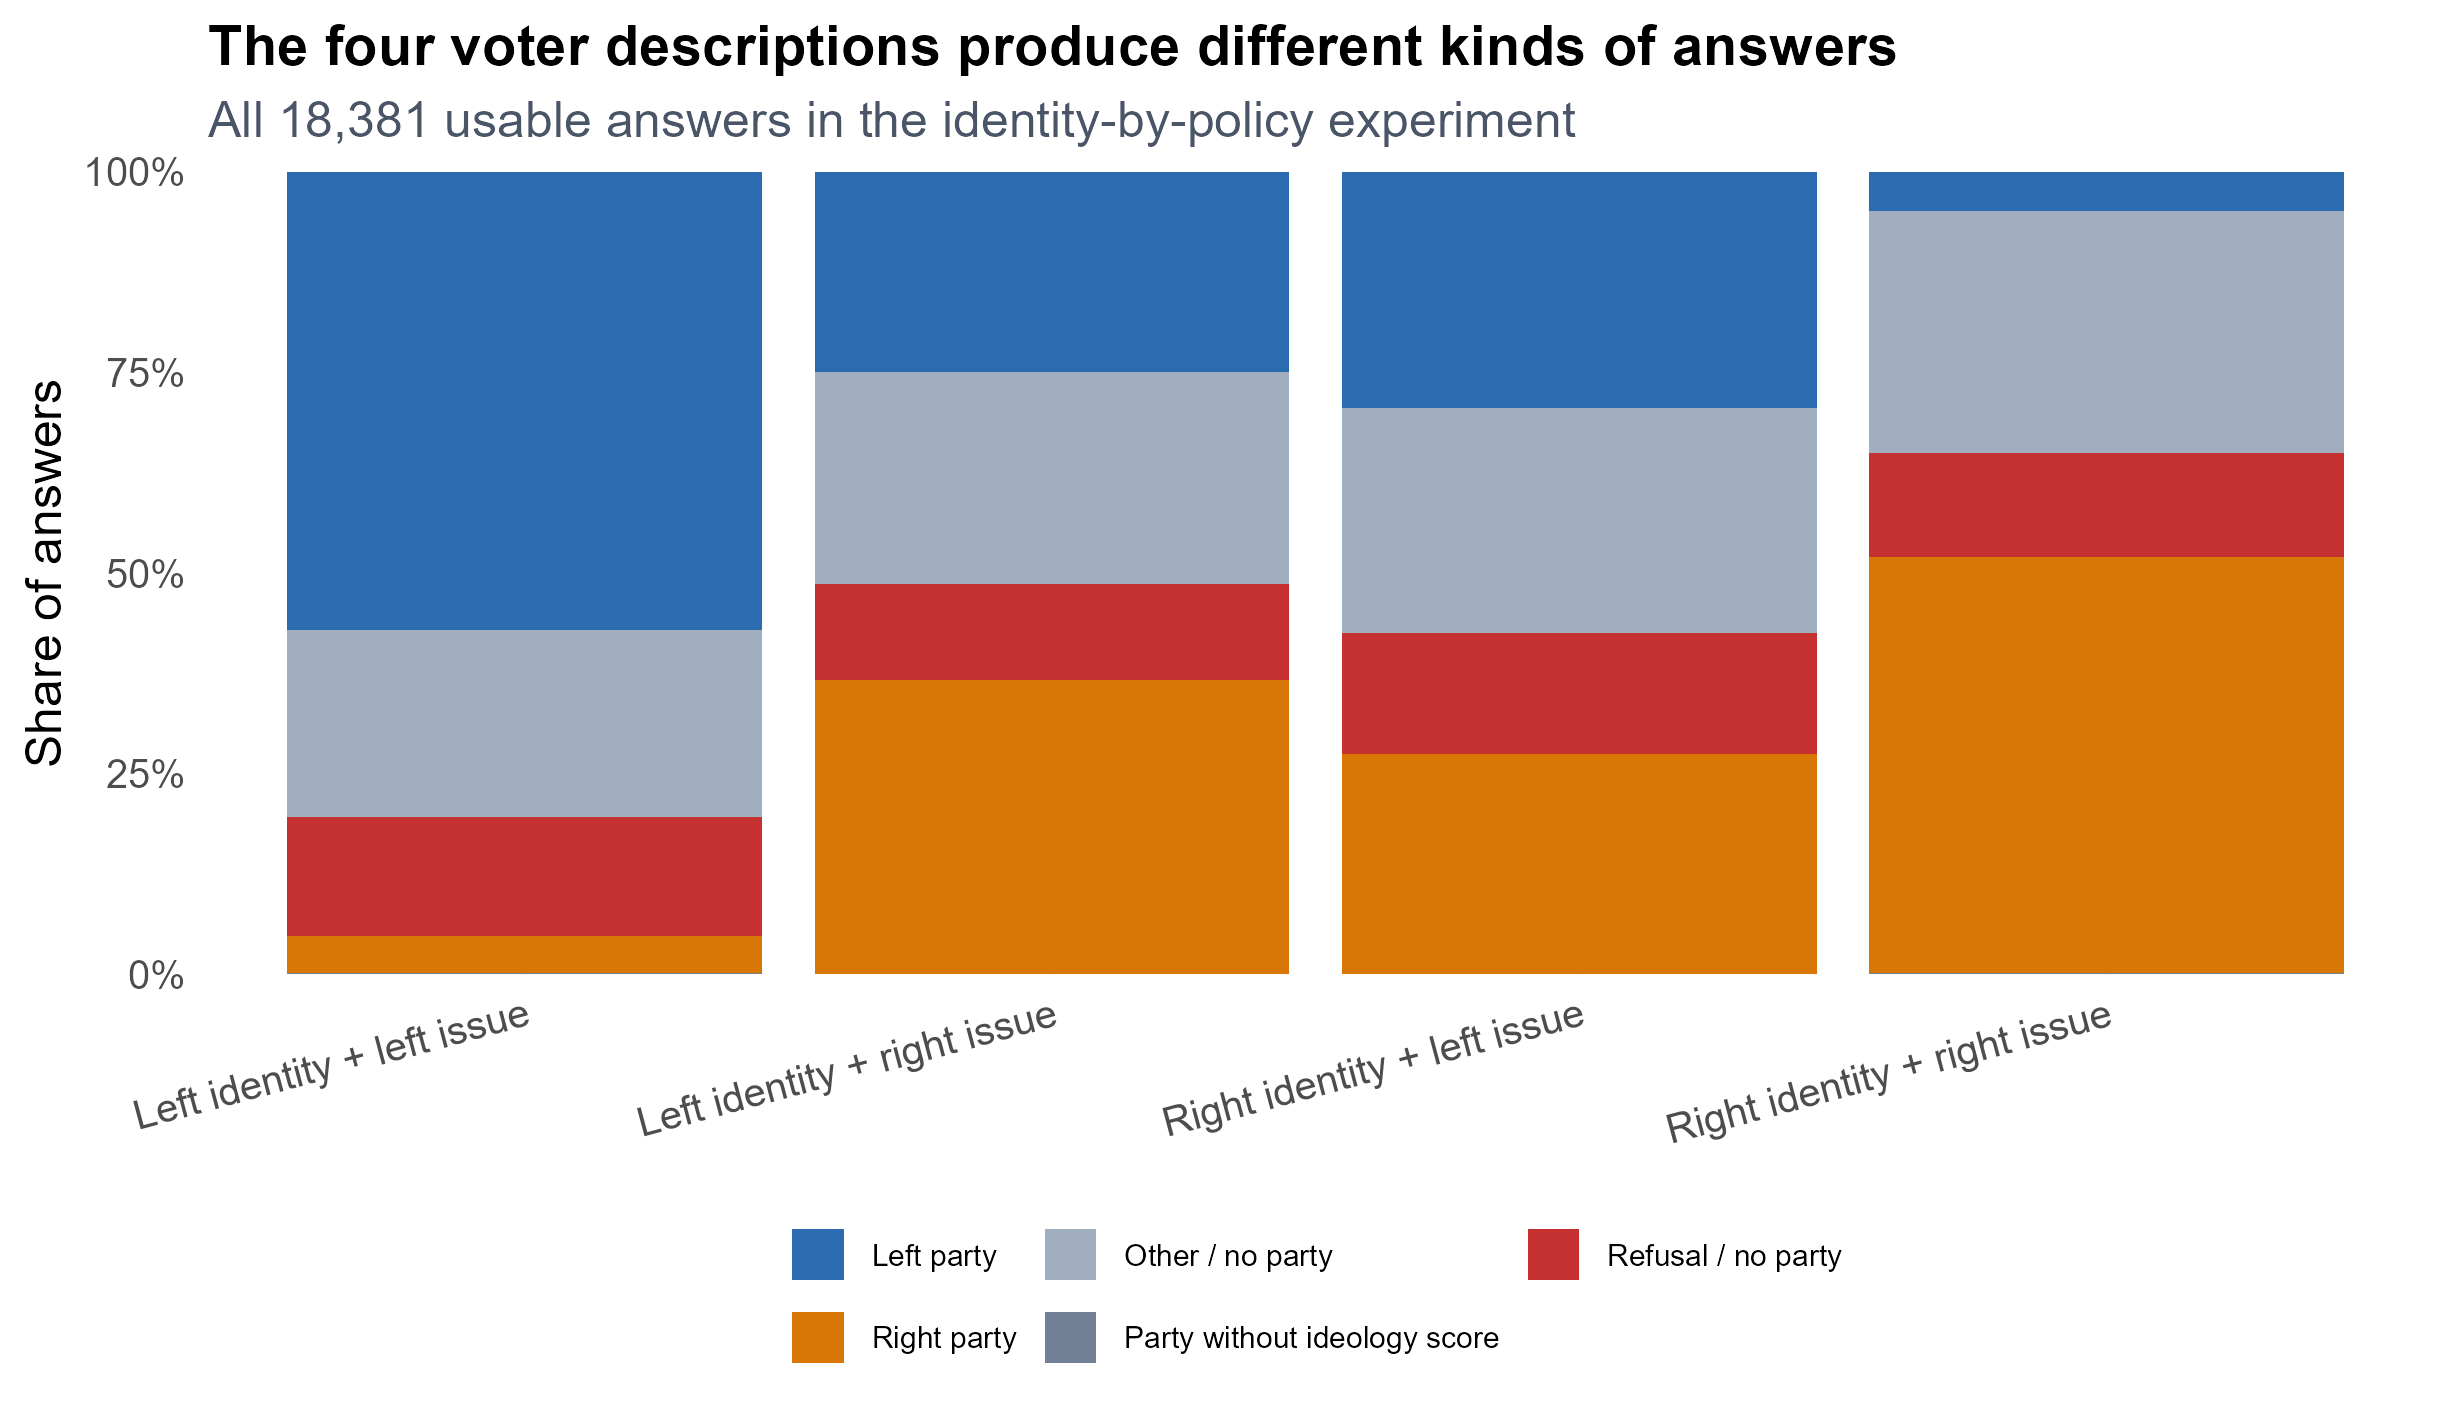
\includegraphics[width=.87\textwidth,height=.60\textheight,keepaspectratio]{01_scenario_distribution.png}\end{center}
\source{Module C, all usable systems, N=18,381. The figure includes refusals and answers without a party.}
\end{frame}

\begin{frame}{When identity and policy agree, the recommendation is much clearer}
\small
\begin{center}
\begin{tabular}{lrrr}\toprule
\textbf{Scenario}&\textbf{Left party}&\textbf{Right party}&\textbf{No party}\\\midrule
Left identity + left policy&57.1\%&4.7\%&38.2\%\\
Left identity + right policy&25.0\%&36.6\%&38.4\%\\
Right identity + left policy&29.4\%&27.3\%&43.2\%\\
Right identity + right policy&4.9\%&51.9\%&43.2\%\\\bottomrule
\end{tabular}
\end{center}
\vspace{.1cm}
Conflict changes both recommendation direction and whether a party with an ideology score appears.
\source{All 18,381 usable Module C responses.}
\end{frame}

\begin{frame}{Identity and policy wording change whether and how chatbots answer}
\begin{center}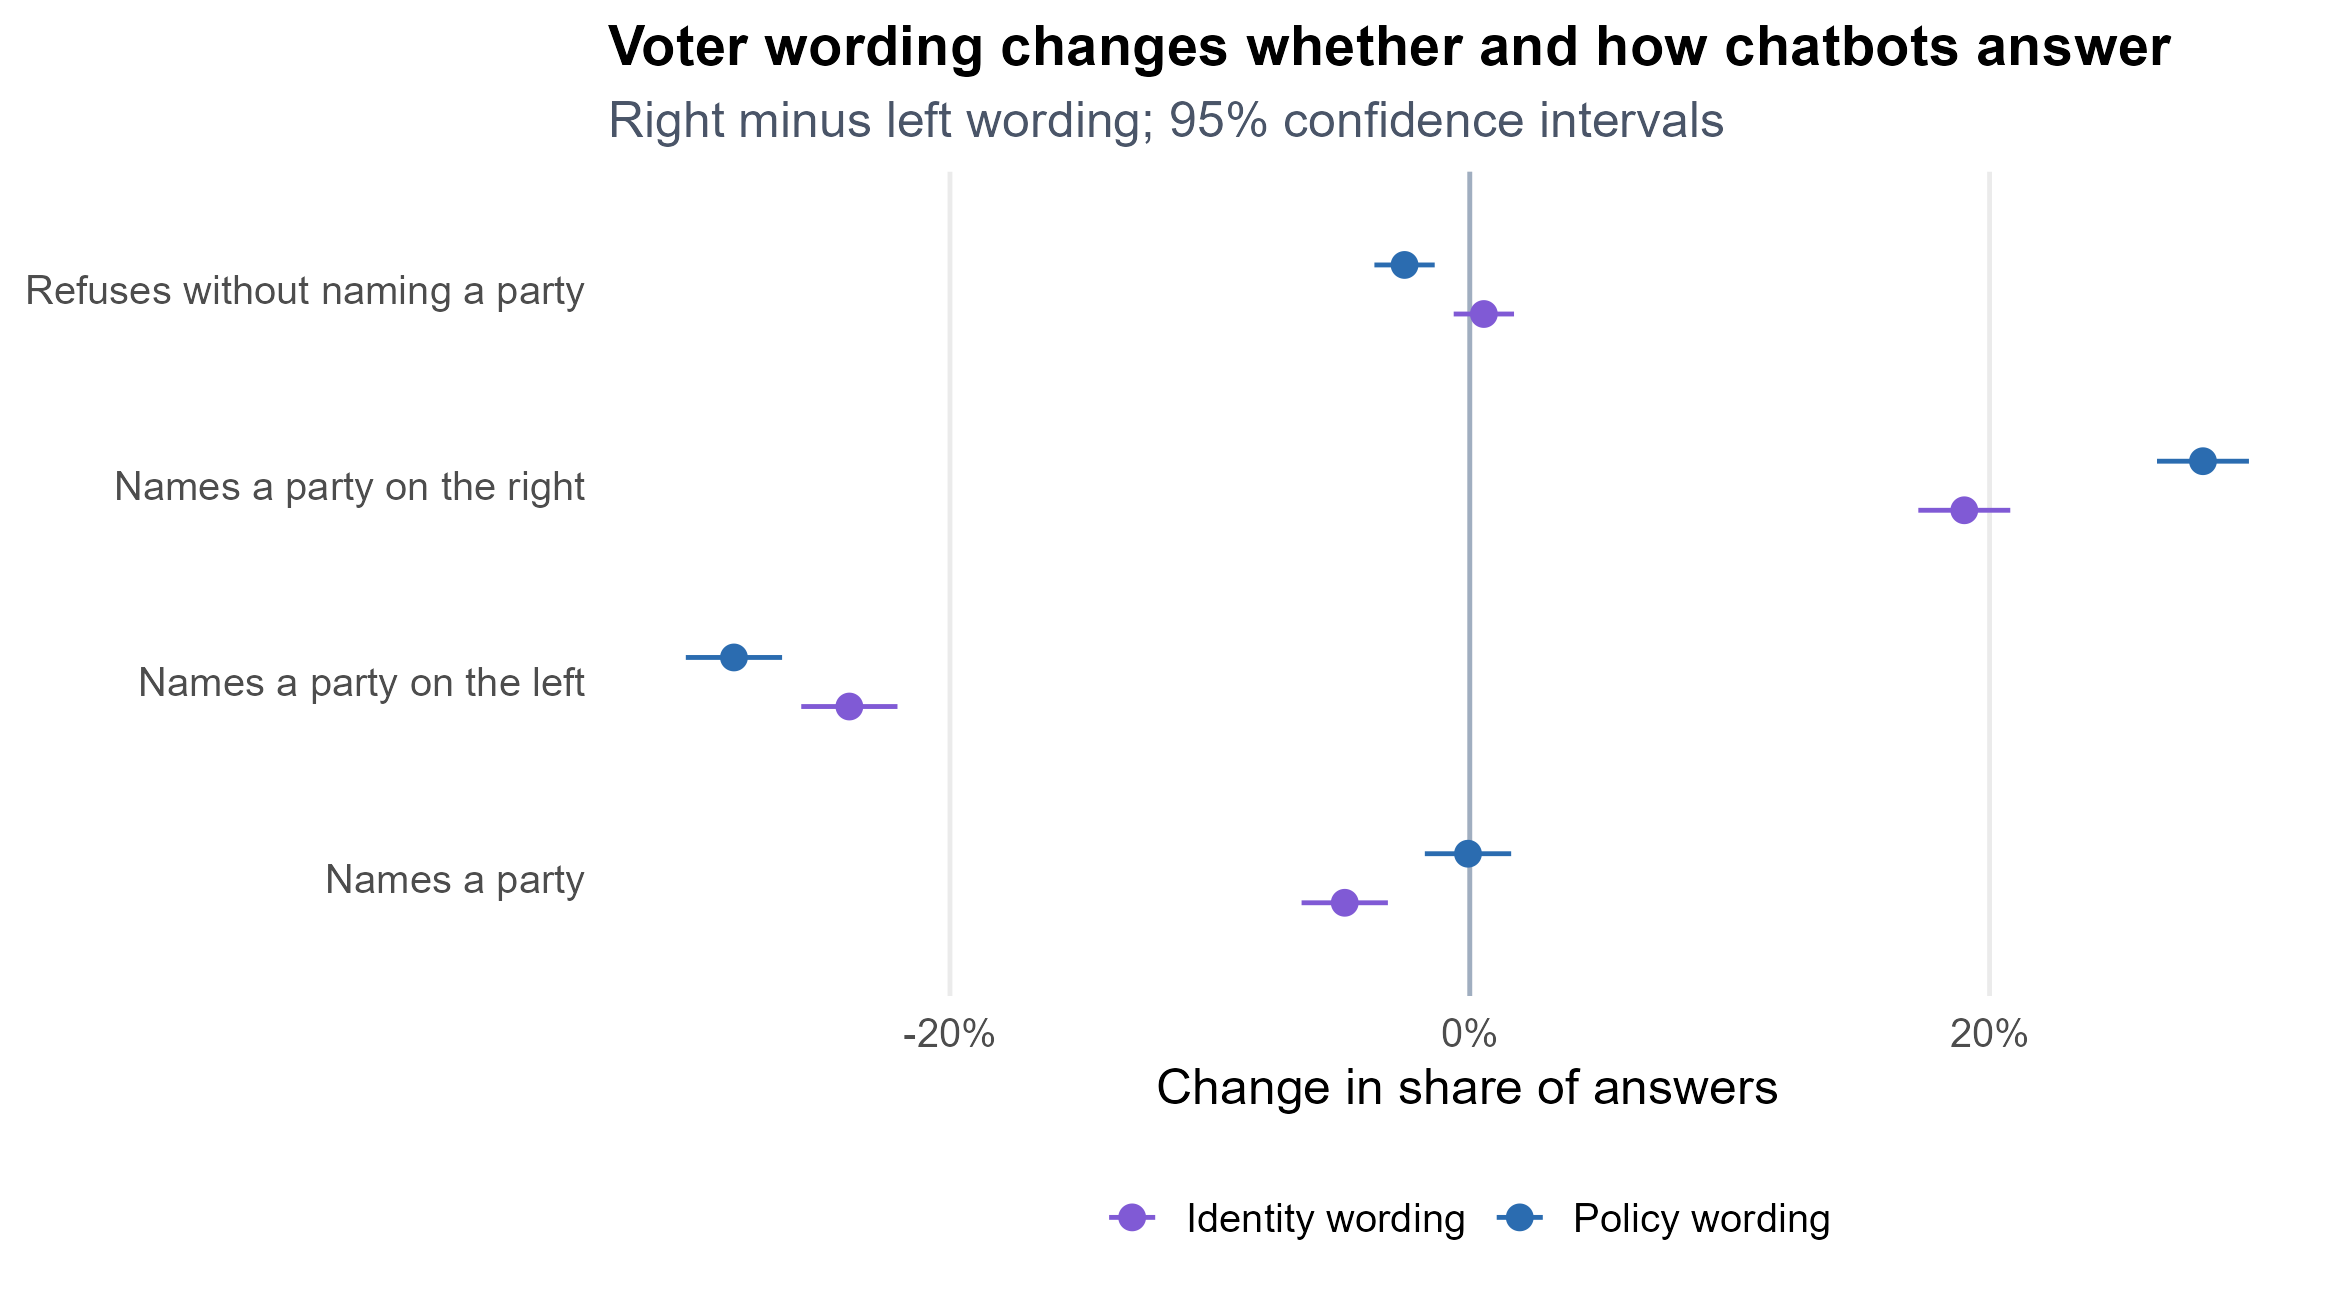
\includegraphics[width=.86\textwidth,height=.60\textheight,keepaspectratio]{02_itt_effects.png}\end{center}
\source{Difference between right and left wording; 95\% confidence intervals account for repeated calls to the same prompt.}
\end{frame}

\begin{frame}{A right-wing identity makes chatbots 4.8 points less likely to name a party}
\begin{columns}[T,onlytextwidth]
\column{.40\textwidth}
\metric{-4.8 pp}{less likely to name a party}
\vspace{.3cm}\par
{\color{muted}95\% confidence interval:\par[-6.5, -3.2] pp}
\column{.54\textwidth}
\begin{itemize}
\item Changing only the policy from left to right does not meaningfully change whether a party is named.
\item If we study only answers that name a party, we miss this difference.
\item This is why the main analysis keeps refusals and answers without a party.
\end{itemize}
\end{columns}
\source{Comparison within chatbot, ballot, and request format; all 18,381 usable Module C answers.}
\end{frame}

\begin{frame}{Both identity and policy move recommendations left or right}
\begin{center}
\begin{tabular}{lrr}\toprule
\textbf{Outcome using all answers}&\textbf{Identity wording}&\textbf{Policy wording}\\\midrule
Names a party on the right&+19.0 pp&+28.2 pp\\
Names a party on the left&-23.9 pp&-28.3 pp\\
Refuses without party&+0.5 pp&-2.5 pp\\\bottomrule
\end{tabular}
\end{center}
\vspace{.35cm}
Across the audited chatbots, both pieces of information move recommendations. The policy wording produces the larger average change.
\end{frame}
\begin{frame}{A second analysis asks how far left or right the named party is}
\[
\text{party score}=\alpha+\beta\,\text{identity}+\gamma\,\text{policy}+\text{controls}
\]
\begin{itemize}
\item $2\beta$ compares the right and left identity descriptions while policy stays fixed.
\item $2\gamma$ compares the right and left policy descriptions while identity stays fixed.
\item The analysis includes only answers naming a party that appears on our ideology scale.
\item It describes party choice after a party is named; it does not describe all chatbot answers.
\end{itemize}
\source{Comparisons are made within chatbot, ballot, and request format; repetitions of the same prompt are grouped together.}
\end{frame}

\begin{frame}{Chatbots differ enormously in how often they name a party}
\footnotesize
\begin{center}
\begin{tabular}{lrr@{\hspace{.65cm}}lrr}\toprule
\textbf{System}&\textbf{Names party}&\textbf{Refusal}&\textbf{System}&\textbf{Names party}&\textbf{Refusal}\\\midrule
Claude Opus&27.5\%&52.2\%&Grok&93.9\%&7.1\%\\
Claude Sonnet&66.5\%&43.2\%&Mistral&96.0\%&1.8\%\\
Gemini Flash&72.3\%&11.5\%&Gemini Pro&4.7\%&4.2\%\\
GPT-4o&45.3\%&3.1\%&DeepSeek&67.1\%&9.6\%\\
Llama&51.5\%&17.7\%&GPT-5&2.2\%&87.5\%\\
Sabi\'a 4&49.6\%&54.1\%&&&\\\bottomrule
\end{tabular}
\end{center}
\vspace{.1cm}
The systems apply very different thresholds for producing a party recommendation.
\source{Rates among all 25,794 usable responses. Refusal/disclaimer and party naming can overlap.}
\end{frame}

\begin{frame}{Among party recommendations, policy moves advice farther than identity}
\begin{center}
\begin{tabular}{lcc}\toprule
\textbf{Part of the prompt}&\textbf{Change on party scale}&\textbf{95\% CI}\\\midrule
Political identity&0.430&[0.402, 0.458]\\
Policy position&0.584&[0.556, 0.612]\\\bottomrule
\end{tabular}
\end{center}
\vspace{.45cm}
This comparison uses 10,890 answers naming a party on the ideology scale. GPT-5 remains in the all-answer analysis but names no scored party in Module C.
\end{frame}

\begin{frame}{Different chatbots rely on identity and policy to different degrees}
\footnotesize
\begin{tabular}{lrr@{\hspace{.7cm}}lrr}\toprule
\textbf{System}&\textbf{Identity}&\textbf{Policy}&\textbf{System}&\textbf{Identity}&\textbf{Policy}\\\midrule
Claude Opus&0.34&0.15&DeepSeek&0.44&0.64\\
Claude Sonnet&0.49&0.39&Gemini Pro&0.84&0.17\\
Gemini Flash&0.39&0.63&Grok&0.42&0.60\\
GPT-4o&0.42&0.70&Mistral&0.35&0.77\\
Llama&0.42&0.61&Sabi\'a 4&0.57&0.51\\\bottomrule
\end{tabular}\par
\vspace{.3cm}
These numbers describe party choice after a party is named. They should be read together with how often each chatbot names a party at all.
\end{frame}

\begin{frame}{For some chatbots, policy matters much more than identity}
\small
For each chatbot, we divide the policy-driven movement by the combined movement associated with policy and identity.
\vspace{.2cm}
\begin{tabular}{lrrrrr}\toprule
System&Opus&Sonnet&Flash&GPT-4o&Llama\\\midrule
Share linked to policy&31\%&45\%&62\%&62\%&59\%\\\bottomrule
\end{tabular}\par
\vspace{.22cm}
\begin{tabular}{lrrrrr}\toprule
System&DeepSeek&Gemini Pro&Grok&Mistral&Sabi\'a 4\\\midrule
Share linked to policy&59\%&17\%&59\%&69\%&47\%\\\bottomrule
\end{tabular}\par
\vspace{.3cm}
This summarizes how far the named party moves. It does not measure whether the recommendation is correct.
\end{frame}

\begin{frame}{When identity and policy conflict, chatbots choose differently}
\footnotesize
\begin{tabular}{lrr@{\hspace{.7cm}}lrr}\toprule
\textbf{System}&\textbf{Policy}&\textbf{Identity}&\textbf{System}&\textbf{Policy}&\textbf{Identity}\\\midrule
Claude Opus&38.6\%&61.4\%&DeepSeek&58.9\%&41.1\%\\
Claude Sonnet&46.1\%&53.9\%&Gemini Pro&13.9\%&86.1\%\\
Gemini Flash&59.6\%&40.4\%&Grok&57.6\%&42.4\%\\
GPT-4o&60.7\%&39.3\%&Mistral&67.4\%&32.6\%\\
Llama&57.1\%&42.9\%&Sabi\'a 4&47.0\%&53.0\%\\\bottomrule
\end{tabular}\par
\vspace{.3cm}
These shares use answers naming a party on the left or right. The earlier chart also includes refusals and answers without a party.
\end{frame}

\begin{frame}{A current party identity matters more than a past vote}
\small
\begin{tabular}{lrr}\toprule
\textbf{Identity formulation}&\textbf{Identity difference}&\textbf{Policy difference}\\\midrule
Party identification&0.76&0.33\\
Ideological self-placement&0.56&0.51\\
Past presidential vote&0.23&0.75\\
Past vote plus indecision&0.14&0.76\\\bottomrule
\end{tabular}\par
\vspace{.35cm}
A current party identity is treated as a stronger signal than electoral history. Explicit indecision makes past vote matter even less.
\end{frame}

\begin{frame}{Policy matters most when users ask for a specific deputy}
\small
\begin{tabular}{lrr}\toprule
\textbf{Context}&\textbf{Identity difference}&\textbf{Policy difference}\\\midrule
Federal deputy, named candidate&0.48&0.72\\
Federal deputy, open advice&0.49&0.55\\
President, named candidate&0.39&0.55\\
President, open advice&0.36&0.53\\\bottomrule
\end{tabular}\par
\vspace{.35cm}
Policy wording produces its largest change when the voter asks for a specific federal-deputy candidate.
\end{frame}

\begin{frame}{Some policy questions produce a wider range of party recommendations}
\begin{itemize}
\item A left Bolsa Fam\'ilia position yields PT in 90.9\% of coded recommendations.
\item A left abortion position is dispersed: PT 45.9\%, PSOL 33.9\%, and PL 13.8\%.
\item A right privatization position yields NOVO in 26.3\% and PL in 62.6\%.
\item A right security position yields PL in 94.0\%.
\end{itemize}
\vspace{.25cm}
The topic matters: some questions spread recommendations across several parties, while others concentrate them on one major party.
\source{Module A, all usable systems, among answers where the script identifies a party.}
\end{frame}

\begin{frame}{We compare chatbots using the same voter descriptions}
\begin{enumerate}
\item For each system and prompt cell, identify the most common answer across repeated calls.
\item Match two systems on prompt cells observed for both.
\item Count how often their most common answers agree.
\end{enumerate}
\vspace{.3cm}
\begin{columns}[T,onlytextwidth]
\column{.47\textwidth}
\key{Broad agreement}
\begin{itemize}
\item same response type
\item same ideological side
\end{itemize}
\column{.47\textwidth}
\key{Exact agreement}
\begin{itemize}
\item same party
\item or same non-party outcome
\end{itemize}
\end{columns}
\source{The reported mean summarizes 45 pairs among systems with at least 354 Module C cells.}
\end{frame}
\begin{frame}{The same voter description usually gets different answers across chatbots}
\begin{columns}[T,onlytextwidth]
\column{.42\textwidth}
\metric{37.7\%}{mean agreement on response side/type}\vspace{.25cm}
\metric{33.9\%}{mean agreement on exact party/type}
\column{.52\textwidth}
\begin{itemize}
\item Each pair compares the same assigned voter descriptions.
\item The comparison covers 10 systems with at least 354 of 384 Module C cells.
\item The most common answer is taken across repeated calls within each cell.
\end{itemize}
\end{columns}
\source{Forty-five system pairs. GPT-5 remains in the all-answer analysis but has only 52 Module C cells.}
\end{frame}

\begin{frame}{Grok and Mistral are the closest pair; Gemini Pro is an outlier}
\small
\begin{tabular}{lrr}\toprule
\textbf{System pair}&\textbf{Same side/type}&\textbf{Same exact party/type}\\\midrule
Grok vs Mistral&75.8\%&59.4\%\\
Gemini Flash vs Mistral&72.4\%&62.5\%\\
Gemini Flash vs Grok&63.3\%&47.1\%\\\midrule
Gemini Pro vs Mistral&4.2\%&4.9\%\\
Gemini Pro vs Sabi\'a 4&4.2\%&4.4\%\\
Gemini Pro vs Grok&2.3\%&2.3\%\\\bottomrule
\end{tabular}\par
\vspace{.3cm}
Gemini Pro rarely names a party, so its most common answer differs sharply from chatbots that usually recommend one.
\end{frame}

\begin{frame}{A rich profile is a fictional voter described with many details}
\begin{itemize}
\item Each profile combines occupation, income, religion, geography, political history, values, and several policy positions.
\item The nine profiles adapt voter groups described in \textit{Brasil no Espelho}.
\item Examples include a left activist, a low-income voter, a social liberal, a solo entrepreneur, a Christian conservative, an agribusiness voter, and a business owner.
\end{itemize}
\vspace{.25cm}
The purpose is to test how chatbots respond to realistic combinations of voter characteristics, not isolated one-line signals.
\source{The profiles are fictional. They do not estimate how real members of these groups would be treated.}
\end{frame}

\begin{frame}{We compare whole profiles; no single characteristic is isolated}
\begin{columns}[T,onlytextwidth]
\column{.47\textwidth}
\key{What changes together}
\begin{itemize}
\item occupation and income
\item identity and past vote
\item religion and values
\item several policy positions
\end{itemize}
\column{.47\textwidth}
\key{What we cannot separate}
\begin{itemize}
\item the effect of race alone
\item the effect of class alone
\item the effect of religion alone
\item the effect of occupation alone
\end{itemize}
\end{columns}
\vspace{.3cm}
A difference between two profiles belongs to the complete descriptions, not to any one characteristic.
\end{frame}

\begin{frame}{The profiles line up with how their source groups voted in 2022}
\begin{center}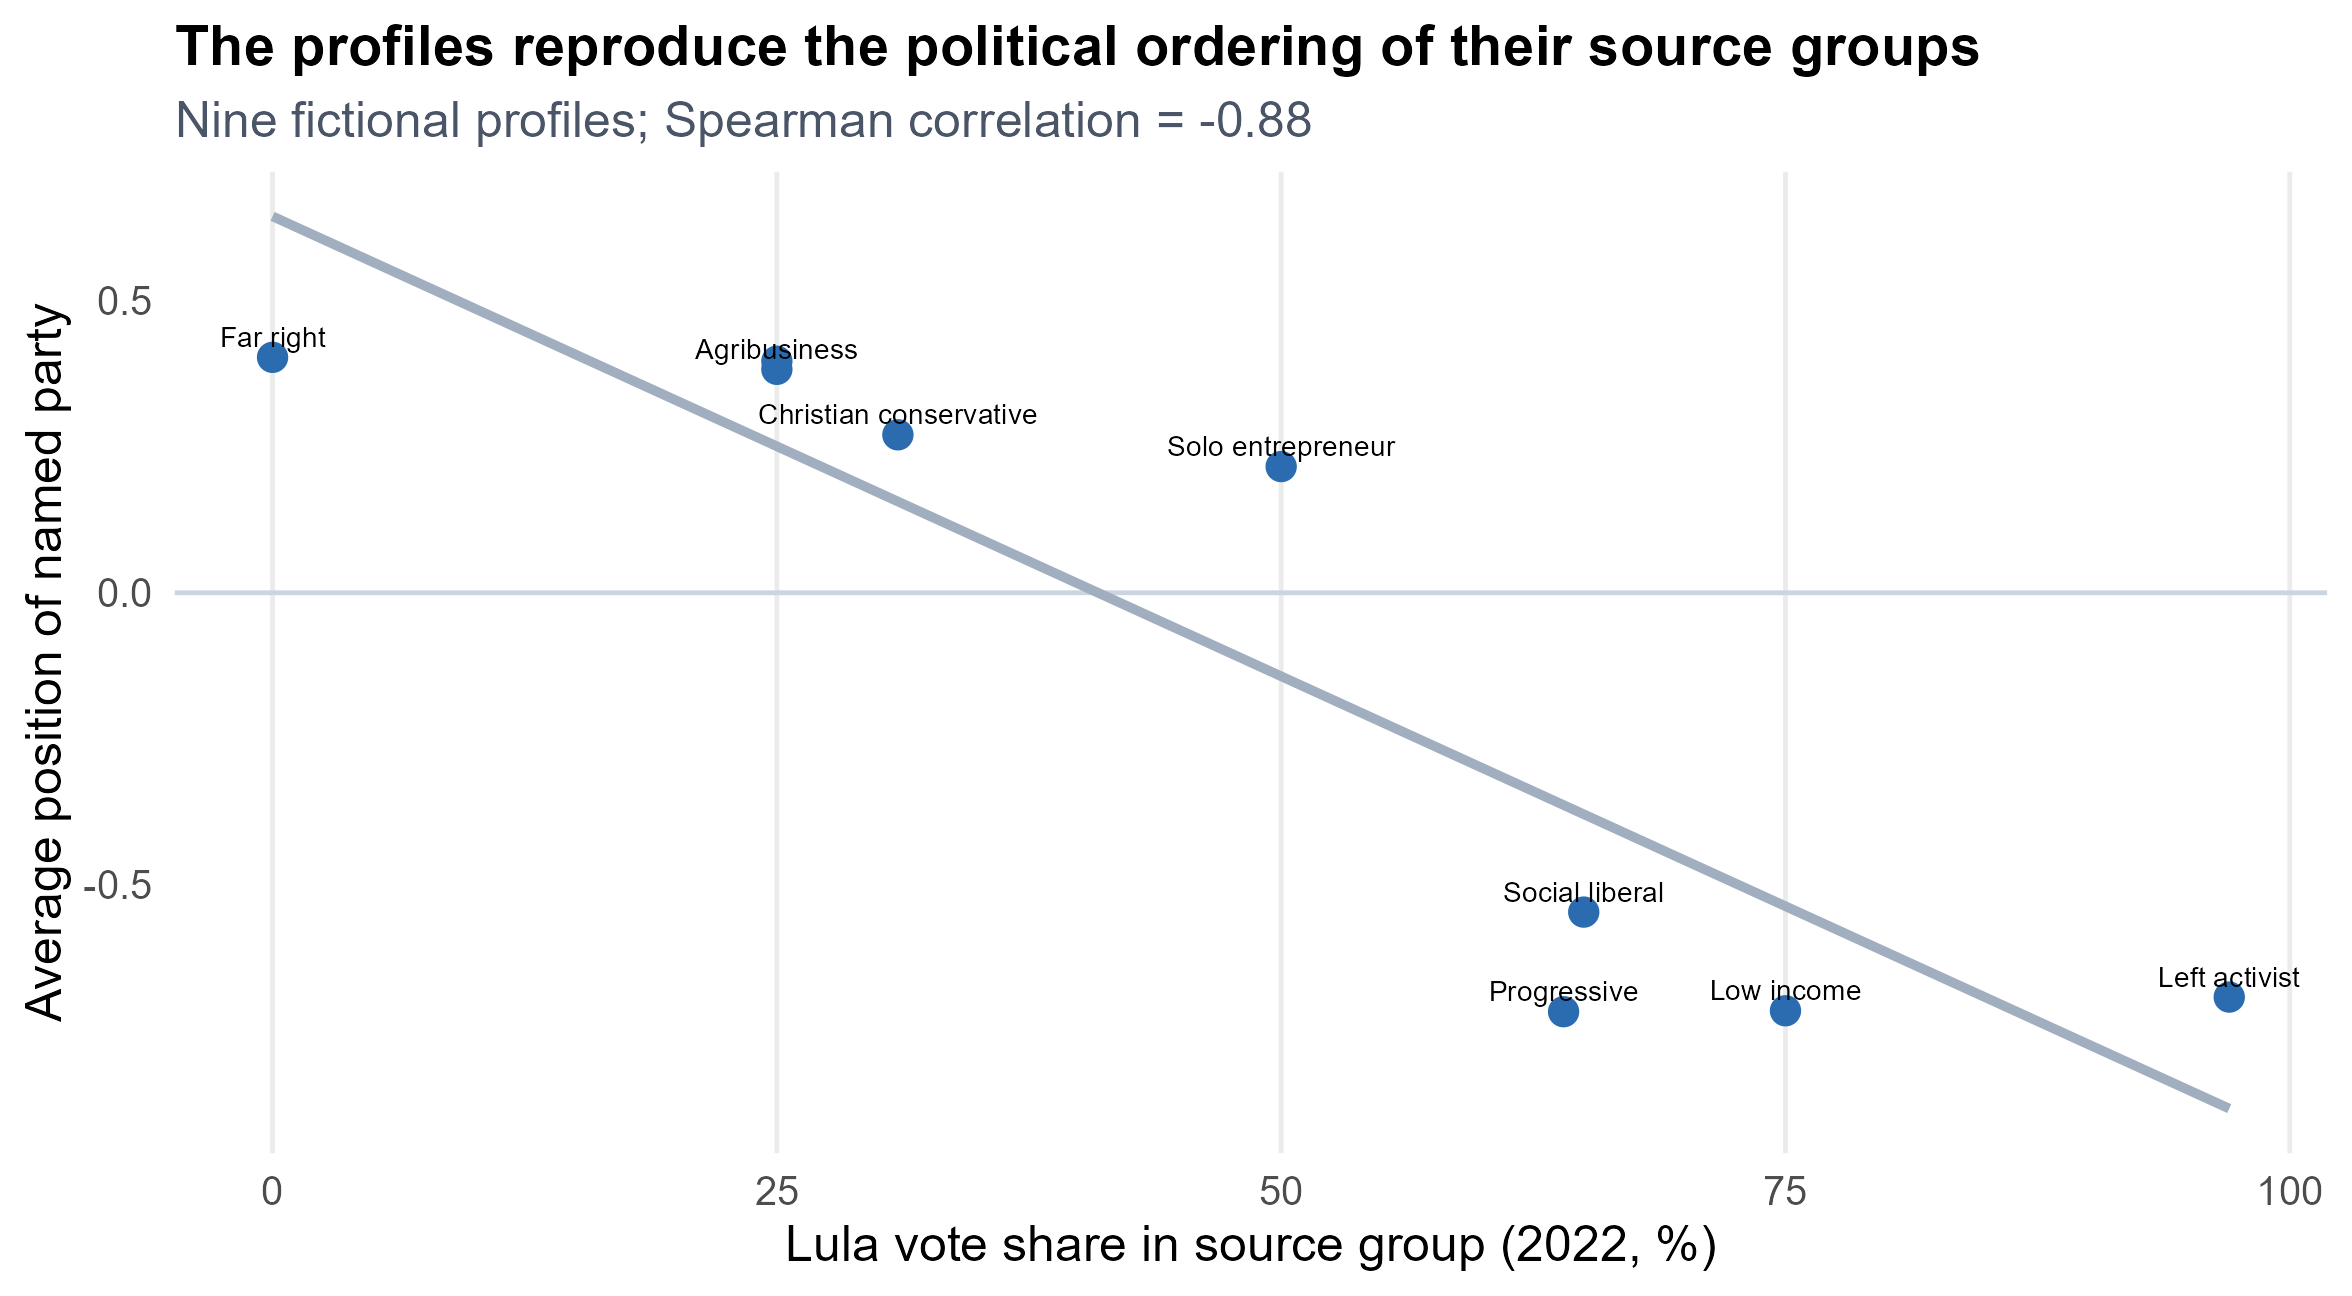
\includegraphics[width=.80\textwidth,height=.60\textheight,keepaspectratio]{05_rich_profile_validation.png}\end{center}
\source{Nine fictional profiles; average position of the named party across chatbots that name a party on the ideology scale.}
\end{frame}

\begin{frame}{Profiles from more pro-Lula groups receive more left-wing recommendations}
\begin{columns}[T,onlytextwidth]
\column{.39\textwidth}
\metric{-0.88}{rank correlation}\vspace{.2cm}
As Lula's 2022 vote share rises in the source group, the average named party moves left.
\column{.55\textwidth}
\begin{itemize}
\item Left activist, low-income, progressive, and social-liberal profiles appear on the left.
\item Agribusiness, Christian conservative, business-owner, and far-right profiles appear on the right.
\item The ordering is plausible, but it does not show that any recommendation is correct or fair.
\end{itemize}
\end{columns}
\source{Nine complete profiles; only answers naming a party on the ideology scale enter the correlation.}
\end{frame}

\begin{frame}{Some profiles are much more likely to receive a party recommendation}
\small
\begin{tabular}{lrr}\toprule
\textbf{Complete profile}&\textbf{Names party}&\textbf{Refusal/disclaimer}\\\midrule
Left activist&86.0\%&4.5\%\\
Social liberal&76.8\%&11.6\%\\
Far right&63.6\%&17.0\%\\
Low-income state-dependent&56.0\%&25.0\%\\
Christian conservative&49.2\%&18.5\%\\\bottomrule
\end{tabular}\par
\vspace{.3cm}
A follow-up experiment should change one profile characteristic at a time to identify which detail drives the answer.
\end{frame}
\begin{frame}{The preta description reduces refusal by 19.6 percentage points}
\begin{center}
\begin{tabular}{lrr}\toprule
\textbf{Description, compared with branca}&\textbf{Refusal/disclaimer}&\textbf{Party named}\\\midrule
Parda&-12.1 pp&+14.6 pp\\
Preta&-19.6 pp&+16.7 pp\\\bottomrule
\end{tabular}
\end{center}
\vspace{.35cm}
In this experiment, both racial descriptions reduce refusal and increase party naming relative to branca. All four confidence intervals exclude zero. Human review of the automated response classification remains important.
\source{All usable Part D answers; comparisons within chatbot, profile step, ballot, and request format.}
\end{frame}

\begin{frame}{The same chatbot often changes its answer across identical calls}
\footnotesize
\begin{tabular}{lr@{\hspace{1cm}}lr}\toprule
\textbf{System}&\textbf{All repeats identical}&\textbf{System}&\textbf{All repeats identical}\\\midrule
Claude Opus&14.1\%&Grok&48.4\%\\
Claude Sonnet&19.3\%&Mistral&60.9\%\\
Gemini Flash&29.9\%&Gemini Pro&84.4\%\\
GPT-4o&26.6\%&DeepSeek&52.5\%\\
Llama&25.8\%&GPT-5&94.2\%\\
Sabi\'a 4&9.6\%&&\\\bottomrule
\end{tabular}\par
\vspace{.3cm}
The outcome combines exact party, refusal, and other response. High agreement can therefore reflect consistently declining or avoiding a party recommendation.
\source{Share of observed Module C cells with identical outcomes across all available repetitions.}
\end{frame}

\begin{frame}{Three findings: the chatbot, the voter description, and repeated calls all matter}
\begin{itemize}
\item \key{Different chatbots:} two systems give the same most common side or answer type in only 37.7\% of matched comparisons.
\item \key{Different wording:} changing identity from left to right makes a party 4.8 percentage points less likely to be named.
\item \key{Same prompt, new call:} many chatbots change the party or answer type across identical requests.
\end{itemize}
\vspace{.4cm}
The result is not one shared left-right bias. Each chatbot applies its own, partly inconsistent way of deciding whether and what to recommend.
\end{frame}

\begin{frame}{What the experiment can tell us}
\begin{itemize}
\item Because identity and policy wording were randomly assigned, average answer differences can be attributed to those wording changes.
\item We can compare the named chatbot versions using the same prompts.
\item We can describe how complete rich profiles are treated.
\item We can measure how often the same chatbot changes its answer across identical calls.
\item These conclusions apply to the prompts, systems, and collection period studied here.
\end{itemize}
\end{frame}

\begin{frame}{What the experiment cannot tell us}
\begin{itemize}
\item Whether chatbot advice changes how real voters vote
\item Whether a recommended party truly matches the stated policy
\item Why one vendor or model family behaves differently
\item Which single characteristic drives a result for a rich profile
\item Whether the same pattern will hold after an interface or model update
\end{itemize}
\end{frame}

\begin{frame}{Why this matters: voting advice changes across chatbots and across calls}
\begin{enumerate}
\item Some chatbots routinely name parties; others usually refuse or avoid doing so.
\item Identity and policy information change both whether a party is named and which side is recommended.
\item The same voter description often produces different answers across chatbots.
\item Even the same chatbot may change its answer when the identical request is repeated.
\end{enumerate}
\vspace{.3cm}
For voters, the platform itself becomes an unobserved part of the advice they receive.
\end{frame}
\begin{frame}{Next: test whether the advice is substantively correct}
\begin{itemize}
\item Have human coders verify refusals, vague answers, parties, and candidates.
\item Link recommended parties and candidates to documented issue positions.
\item Compare each recommendation with the policy position stated by the voter.
\item Model the two decisions together: whether to name a party and which party to name.
\item Repeat the study within a fixed model-version window to measure change over time.
\end{itemize}
\vspace{.35cm}
This pilot shows that policy information changes advice. The next question is whether the resulting advice is accurate.
\end{frame}

\begin{frame}{References}\footnotesize
\begin{thebibliography}{9}
\bibitem{bolognesi} Bolognesi, Ribeiro, and Codato. 2023. ``Classifica\c{c}\~ao ideol\'ogica dos partidos pol\'iticos brasileiros.'' \textit{Dados} 66(2).
\bibitem{miyazaki} Miyazaki and Hall. 2026. ``Why Do AI Models Tell Left-Wing Voters to Support the Communist Party?'' Working paper.
\bibitem{neto} Neto. 2024. \textit{Brasil no Espelho}. Quaest, chapter 8.
\bibitem{zucco} Zucco and Power. 2024. Brazilian Legislative Surveys, waves 1--9. \textit{Latin American Politics and Society} 66(1), appendix C.
\end{thebibliography}
\vfill{\fontsize{9}{11}\selectfont\color{muted}All empirical results are authors' calculations from the July 2026 S\~ao Paulo pilot.}
\end{frame}
\end{document}
